\chapter{Пошук карти глибин за стереопарою}

Другий розділ присвячено розв'язку задачі стереобачення алгоритмом дифузії.
Описуються властивості алгоритму та з'ясовується придатність
розв'язку для поставленої задачі.

\section{Відомості з теорії оптимізації}
Введемо декілька визначень та тверджень \cite{overview:savchynskyy:diffusion},
що знадобляться при розв'язанні задачі.

\textbf{Означення.}
\textit{Опуклим бакатогранником} (polyhedron) $P$ в $\mathbb{R}^n$ називається множина,
що може бути представлена скінченним набором лінійних нерівностей,
тобто
$P = \left\{
    \pmb{x} \in \mathbb{R}^n \; \middle| \;
    \hat{A} \cdot \pmb{x} \le \pmb{b}
\right\}$
для матриці $\hat{A} \in \mathbb{R}^{m \times n}$ і вектору
$\pmb{b} \in \mathbb{R}^n$.
Обмежений опуклий багатогранник називається \textit{політопом} (polytope).

\textbf{Означення.}
Політоп
\begin{equation} \label{eq:simplex}
    \Delta^n := \left\{
    \pmb{x} \in \mathbb{R}^n_+ \; \middle| \; \sum \limits_{x = 1}^n x_i = 1
    \right\}
\end{equation}
називається \textit{$n$-вимірним (ймовірнісним) симплексом}.

\textbf{Означення.}
Для множини $X \subset \mathbb{R}^n$ множина
\begin{equation*}
    conv \left(X \right) = \left\{
        \pmb{s} \in \mathbb{R}^n \; \middle| \;
        \exists N \in \mathbb{N}_+ \; : \;
        s = \sum \limits_{i = 1}^N p_i \cdot x^i, \,
        x_i \in X, \,
        \pmb{p} \in \Delta^N
    \right\}
\end{equation*}
точок,
які представлені як опукла комбінація скінченного числа точок з множини $X$,
називається \textit{опуклою оболонкою} множини $X$.

\textbf{Означення.}
Нехай $P$~---~опуклий багатогранник в $\mathbb{R}^n$,
визначений множиною лінійних обмежень.
Оптимізаційні задачі виду
\begin{equation*}
    \min \limits_{\pmb{x} \in P} \langle \pmb{c}, \pmb{x} \rangle, \qquad
    \max \limits_{\pmb{x} \in P} \langle \pmb{c}, \pmb{x} \rangle
\end{equation*}
називаються \textit{задачами лінійного програмування}.

\textbf{Означення.}
Задача лінійного програмування з додатковим обмеженням,
яке дозволяє всім змінним приймати значення тільки $0$ або $1$,
наприклад,
\begin{equation*}
    \min \limits_{\pmb{x} \in P \cap \left\{ 0, 1 \right\}^n}
    \langle \pmb{c}, \pmb{x} \rangle,
\end{equation*}
називається \textit{задачею булевого цілочисельного лінійного програмування}.

\textbf{Означення.}
Нехай задача
\begin{equation} \label{eq:minimization:problem}
    \min_{\pmb{x} \in X} f \left( \pmb{x} \right)
\end{equation}
є задачею мінімізації функції $f: X \to \mathbb{R}$ на множині
$X \subseteq \mathbb{R}^n$.
Тоді оптимізаційна задача
\begin{equation*}
    \min_{\pmb{x} \in X'} g \left(\pmb{x} \right)
\end{equation*}
називається \textit{релаксацією} задачі \eqref{eq:minimization:problem},
якщо $X' \supseteq X$ та $g \left( \pmb{x} \right) \ge f \left( \pmb{x} \right)$
для будь-якого $\pmb{x} \in X$.

\textbf{Означення.}
Для задачі \eqref{eq:minimization:problem} множина $X$ називається
\textit{допустимою множиною}, а $\pmb{x} \in X$~---~\textit{допустимою точкою}.

\textbf{Означення.}
Розглянемо задачу цілочисельного лінійного програмування
\begin{equation} \label{eq:ILP}
    \min \limits_{\substack{\pmb{x} \in P \cap \left\{ 0, 1\right\}^n \\
                  \hat{A} \cdot \pmb{x} = \pmb{b}}}
        \langle \pmb{c}, \pmb{x} \rangle,
\end{equation}
де $P$~---~політоп, $\hat{A} \in \mathbb{R}^{m \times n}$,
$\pmb{b} \in \mathbb{R}^n$.

\textit{Дуальна функція Лагранжа} для задачі \eqref{eq:ILP} має вигляд
\begin{equation} \label{eq:dualization}
    \min \limits_{\pmb{x} \in P \cap \left\{ 0, 1 \right\}^n}
        \langle \pmb{c}, \pmb{x} \rangle +
        \langle \pmb{\lambda}, \hat{A} \cdot \pmb{x} - \pmb{b} \rangle, \qquad
    \pmb{\lambda} \in \mathbb{R}^n.
\end{equation}
Змінна $\pmb{\lambda}$ називається \textit{дуальною змінною}.
Цей прийом називається \textit{дуалізацією обмежень}
$\hat{A} \cdot \pmb{x} = \pmb{b}$,
а релаксації такого вигляду називаються \textit{лагранжевими релаксаціями}.
Наступна задача є дуальною задачею Лагранжа для задачі \eqref{eq:ILP}
\begin{equation} \label{eq:lagrange:dual:problem}
    \max \limits_{\pmb{\lambda} \in \mathbb{R}^n}
        \min \limits_{\pmb{x} \in P \cap \left\{ 0, 1 \right\}^n}
            \langle \pmb{c}, \pmb{x} \rangle +
            \langle \pmb{\lambda}, \hat{A} \cdot \pmb{x} - \pmb{b} \rangle.
\end{equation}

\textbf{Твердження.}
(Прямо-двоїсті умови оптимальності, Primal-dual optimality conditions)
Вектор $\pmb{\lambda}^*$~---~це оптимум дуальної задачі
\eqref{eq:lagrange:dual:problem} тоді й тільки тоді, коли існує
\begin{equation} \label{eq:primal:dual:optimality:condition}
\begin{gathered}
    \pmb{x}^* \in
    \arg\,\min \limits_{\pmb{x} \in conv \left( P \cap \left\{ 0, 1\right\}^n\right)}
        \langle \pmb{c}, \pmb{x} \rangle +
        \langle \pmb{\lambda}, \hat{A} \cdot \pmb{x} - \pmb{b} \rangle = \\
    = \arg\,\min \limits_{\pmb{x} \in conv \left( P \cap \left\{ 0, 1\right\}^n\right)}
        \langle \pmb{c} + \hat{A}^T \cdot \pmb{\lambda}, \pmb{x} \rangle,
\end{gathered}
\end{equation}
такий що $\hat{A} \cdot \pmb{x}^* = \pmb{0}$.
Іншими словами, $\pmb{\lambda}^*$~---~це дуальний оптимум тоді й тільки тоді,
коли існує такий $\pmb{x}^*$,
що задовольняє \eqref{eq:primal:dual:optimality:condition}
і є допустимим для релаксованої прямої задачі
\begin{equation*}
    \min \limits_{\substack{\pmb{x} \in conv \left( P \cap \left\{ 0, 1 \right\}^n\right) \\
                            \hat{A} \cdot \pmb{x} = \pmb{b}}}
        \langle \pmb{c}, \pmb{x} \rangle.
\end{equation*}
Такий $\pmb{x}^*$ є розв'язком релаксованої прямої задачі.

\textbf{Примітка.}
Якщо крім виконання умови \eqref{eq:primal:dual:optimality:condition} та
$\hat{A} \cdot \pmb{x}^* = \pmb{0}$ справедливо,
що $\pmb{x}^* \in \left\{ 0, 1 \right\}^n$,
тоді $\pmb{x}^*$~---~це розв'язок нерелаксованої
цілочисельної задачі лінійного програмування \eqref{eq:ILP}.

\section{Релаксація Лагранжа для поставленої оптимізаційної задачі}

Введемо вектор $\pmb{\mu}$, який містить змінну з множини $ \left[ 0, 1 \right]$
для кожної вершини
$\left( x, y, d \right), \left(x, y \right) \in T, d \in D$ та кожної дужки
$\left( \left( x, y, d \right), \left(x', y', d' \right) \right)$,
що поєднує пари міток $d, d' \in D$ між сусідніми об'єктами
$\left(\left(x, y \right), \left(x', y' \right) \right) \in \mathcal{N}$
в побудованому графі.
Множину всіх вершин і дужок графу позначимо через $\mathcal{I}$.

Елементи даного вектору $\mu_{\left(x, y \right)} \left(d \right)$,
що відповідають вершинам, мають бути узгодженими з розміткою $\pmb{d}$,
тобто якщо $\mu_{\left(x, y \right)} \left(d^* \right) = 1$ для якоїсь мітки
$d^* \in D$,
то $d \left(x, y \right) = d^*$.
Розмітка $\pmb{d}$, за визначенням,
має в кожному об'єкті $\left(x, y \right) \in T$
обрати одну й тільки одну мітку $d \in D$.
Таким чином, на елементи вектора $\pmb{\mu}$
накладаються \textit{обмеження однозначності для вершин} в об'єкті
\begin{equation} \label{eq:vetrex:unambiguity}
    \sum \limits_{d \in D} \mu_{\left( x, y \right)} \left( d \right) = 1,
    \qquad \forall \left(x, y \right) \in T,
\end{equation}
тобто у випадку, якщо вектор $\pmb{\mu}$~---~бінарний,
то тільки один його елемент,
що відповідає вершинам в об'єкті $\left(x, y \right)$, може бути рівним одиниці.

Якщо в об'єкті обрана вершина $d^*$, то обрані дужки,
що виходять із даного об'єкту до сусідніх об'єктів,
мають виходити з цієї ж вершини (рис.~\ref{fig:combining:constraints}).
Ці обмеження називаються \textit{поєднуючими}
\begin{equation} \label{eq:combining:constraints}
    \sum \limits_{d \in D}
        \mu_{\left(x, y \right), \left(x', y' \right)} \left(d, d' \right) =
        \mu_{\left(x', y' \right)} \left(d' \right), \qquad
    \forall
    \left( \left(x, y \right), \left(x',y' \right) \right) \in \mathcal{N},
    d' \in D.
\end{equation}

\begin{figure}[h]
  \centering
  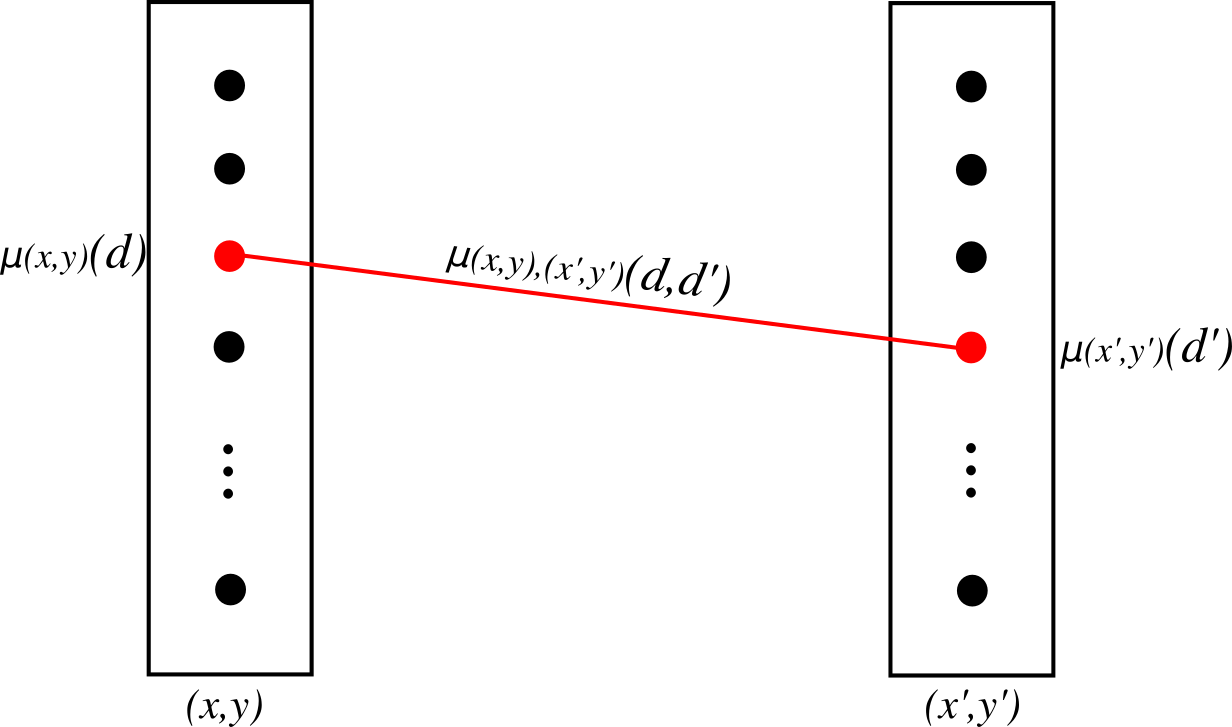
\includegraphics[width=0.7\textwidth]{images/combining_constraints}
  \caption{Поєднуючі обмеження}
  \label{fig:combining:constraints}
\end{figure}

З цих обмежень також випливає,
що між двома сусідніми об'єктами може бути обрана лише одна дужка,
тобто на вектор $\pmb{\mu}$
ще накладаються \textit{обмеження однозначності для дужок}
між парами сусідніх об'єктів
\begin{equation} \label{eq:edge:unambiguity}
    \sum \limits_{d, d' \in D}
        \mu_{\left(x, y \right), \left(x', y' \right)} \left(d, d' \right) = 1,
        \qquad \forall
        \left(\left(x, y \right), \left(x', y' \right) \right) \in \mathcal{N}.
\end{equation}

Обмеження \eqref{eq:vetrex:unambiguity}, \eqref{eq:combining:constraints} та
\eqref{eq:edge:unambiguity} утворюють \textit{локальний політоп}
\begin{equation} \label{eq:local:polytop}
\begin{gathered}
    \mathcal{L} :=
    \begin{cases}
        \sum \limits_{d \in D}
            \mu_{\left(x, y \right), \left(x', y' \right)} \left(d, d' \right) =
            \mu_{\left(x', y' \right)} \left(d' \right), \;
        \forall
        \left( \left(x, y \right), \left(x',y' \right) \right) \in \mathcal{N},
        d' \in D, \\
        \sum \limits_{d \in D} \mu_{\left( x, y \right)} \left( d \right) = 1,
        \qquad \forall \left(x, y \right) \in T, \\
        \sum \limits_{d, d' \in D}
            \mu_{\left(x, y \right), \left(x', y' \right)} \left(
                d, d'
            \right) = 1, \qquad \forall
            \left(\left(x, y \right), \left(x', y' \right) \right) \in
                \mathcal{N}, \\
        \pmb{\mu} \ge \pmb{0},
    \end{cases}
\end{gathered}
\end{equation}
де остання нерівність означає, що кожен елемент вектора $\pmb{\mu}$ невід'ємний.

Отримаємо задачу цілочисельного лінійного програмування
\begin{equation*}
    \min \limits_{\pmb{d} \in D^T} E \left( \pmb{d} \right) =
    \min \limits_{\pmb{\mu} \in \mathcal{L} \cap \left\{ 0, 1 \right\}^{\mathcal{I}}}
        \langle \pmb{\theta}, \pmb{\mu} \rangle,
\end{equation*}
де $\pmb{\theta}$~---~вектор штрафів, накладених на всі вершини та дуги,
елементи якого розташовані в тій же послідовності,
що й елементи вектора $\pmb{\mu}$.

Випишемо скалярний добуток у правій частині останнього виразу в явному вигляді
\begin{equation} \label{eq:ILP:MAP:inference}
\begin{gathered}
    \min \limits_{\pmb{\mu} \in \mathcal{L} \cap \left\{ 0, 1 \right\}^{\mathcal{I}}}
        \langle \pmb{\theta}, \pmb{\mu} \rangle =
    \min \limits_{\pmb{\mu} \in \mathcal{L} \cap \left\{ 0, 1 \right\}^{\mathcal{I}}}
        \left[
            \sum \limits_{\left(x, y \right) \in T}
                \sum \limits_{d \in D}
                    \mu_{\left(x, y \right)} \left(d \right) \cdot
                    f_{\left(x, y \right)} \left( d \right) + \right. \\
            + \left.
            \sum \limits_{\left(\left(x, y \right), \left(x', y' \right) \right) \in \mathcal{N}}
                \sum \limits_{d, d' \in D}
                    \mu_{\left(x, y \right), \left(x', y' \right)} \left(
                        d, d'
                    \right) \cdot
                    g_{\left(x, y \right), \left(x', y' \right)} \left(
                        d, d'
                    \right)
        \right].
\end{gathered}
\end{equation}

Використаємо прийом дуалізації \eqref{eq:dualization}
поєднуючих обмежень \eqref{eq:combining:constraints}
в задачі \eqref{eq:ILP:MAP:inference}.
Новий доданок має вигляд
\begin{equation} \label{eq:dualized:term}
    \sum \limits_{\left(x, y \right) \in T}
        \sum \limits_{\left(x', y' \right) \in \mathcal{N} \left(x, y \right)}
            \sum \limits_{d \in D}
                \varphi_{\left(x, y \right), \left(x', y' \right)} \left(
                    d
                \right) \cdot \left[
                    \sum \limits_{d' \in D}
                        \mu_{\left(x, y \right), \left(x', y' \right)} \left(
                            d, d'
                        \right) - \mu_{\left(x, y \right)} \left(d \right)
                \right],
\end{equation}
де змінні
$\varphi_{\left(x, y \right), \left(x', y' \right)} \left( d \right) \in
    \mathbb{R}$,
$\left(x, y \right) \in T$,
$\left(x', y' \right) \in \mathcal{N} \left(x, y \right)$,
$d \in D$,
є дуальними.
Будемо називати їх \textit{потенціалами} (рис.~\ref{fig:phi:block}).

\begin{figure}[h]
  \centering
  \includegraphics[width=0.6\textwidth]{images/phi_block}
  \caption{Змінна $\varphi_{\left(x, y \right), \left(x', y' \right)} \left(d \right)$}
  \label{fig:phi:block}
\end{figure}

Запишемо цільову функцію задачі \eqref{eq:ILP:MAP:inference}
з урахуванням нового доданку \eqref{eq:dualized:term}, в якому розкриємо дужки
\begin{equation*}
\begin{gathered}
    \langle \pmb{\theta}^{\varphi}, \pmb{\mu} \rangle =
    \sum \limits_{\left(x, y \right) \in T}
        \sum \limits_{d \in D}
            \mu_{\left(x, y \right)} \left(d \right) \cdot
            f_{\left(x, y \right)} \left( d \right) + \\
    + \sum \limits_{\left(\left(x, y \right), \left(x', y' \right) \right) \in \mathcal{N}}
        \sum \limits_{d, d' \in D}
            \mu_{\left(x, y \right), \left(x', y' \right)} \left(
                d, d'
            \right) \cdot
            g_{\left(x, y \right), \left(x', y' \right)} \left(
                d, d'
            \right) + \\
    + \sum \limits_{\left(x, y \right) \in T}
        \sum \limits_{\left(x', y' \right) \in \mathcal{N} \left(x, y \right)}
            \sum \limits_{d \in D}
                \varphi_{\left(x, y \right), \left(x', y' \right)} \left(
                    d
                \right) \cdot
                \sum \limits_{d' \in D}
                    \mu_{\left(x, y \right), \left(x', y' \right)} \left(
                        d, d'
                    \right) - \\
    - \sum \limits_{\left(x, y \right) \in T}
        \sum \limits_{\left(x', y' \right) \in \mathcal{N}\left(x, y \right)}
            \sum \limits_{d \in D}
                \varphi_{\left(x, y \right), \left(x', y' \right)} \left(
                    d
                \right) \cdot \mu_{\left(x, y \right)} \left(d \right).
\end{gathered}
\end{equation*}
Згрупуємо перший доданок з останнім, а другий~---~з третім
\begin{equation} \label{eq:grouped:for:reparametrization}
\begin{gathered}
    \langle \pmb{\theta}^{\varphi}, \pmb{\mu} \rangle =
    \sum \limits_{\left(x, y \right) \in T}
        \sum \limits_{d \in D}
            \mu_{\left(x, y \right)} \left(d \right) \cdot \left[
                f_{\left(x, y \right)} \left(d \right) -
                \sum \limits_{\left(x', y' \right) \in \mathcal{N} \left(x, y \right)}
                    \varphi_{\left(x, y \right), \left(x', y' \right)} \left(
                        d
                    \right)
            \right] + \\
    + \sum \limits_{\left(\left(x, y \right), \left(x', y' \right)\right)\in \mathcal{N}}
        \sum \limits_{d, d' \in D}
             \mu_{\left(x, y \right), \left(x', y' \right)} \left(d, d' \right)
             \cdot \left[
                g_{\left(x, y \right), \left(x', y' \right)} \left(d, d' \right) + \right. \\
                + \left. \varphi_{\left(x, y \right), \left(x', y' \right)} \left(
                    d
                \right) +
                \varphi_{\left(x', y' \right), \left(x, y \right)} \left(
                    d'
                \right)
             \right].
\end{gathered}
\end{equation}

Введемо позначення для \textit{репараметризованого штрафу за вибір мітки}
$d \in D$ в об'єкті $\left(x, y \right) \in T$
\begin{equation} \label{eq:reparametrized:vertex}
    f_{\left(x, y \right)}^{\varphi} \left(d \right) =
    f_{\left(x, y \right)} \left(d \right) -
    \sum \limits_{\left(x', y' \right) \in \mathcal{N} \left(x, y \right)}
        \varphi_{\left(x, y \right), \left(x', y' \right)} \left(
            d
        \right),
\end{equation}
тобто репараметризований
штраф у вершині отримується шляхом віднімання потенціалів,
що виходять із даної вершини в усі сусідні об'єкти,
від вихідного штрафу в вершині (рис.~\ref{fig:reparametrized:vertex:weight}).

\begin{figure}[h]
  \centering
  \includegraphics[width=0.7\textwidth]{images/reparametrized_vertex_weight}
  \caption{Потенціали, які віднімаються від вихідного штрафу в вершині $\left(x, y, d \right)$}
  \label{fig:reparametrized:vertex:weight}
\end{figure}

Також введемо позначення для
\textit{репараметризованого штрафу за вибір пари міток}
$d, d' \in D$ у двох сусідніх об'єктах
$\left( \left(x, y \right), \left(x', y'\right) \right) \in \mathcal{N}$
\begin{equation} \label{eq:reparametrized:edge}
    g_{\left(x, y \right), \left(x', y'\right)}^{\varphi} \left(d, d' \right) =
    g_{\left(x, y \right), \left(x', y' \right)} \left(d, d' \right) +
    \varphi_{\left(x, y \right), \left(x', y' \right)} \left( d \right) +
    \varphi_{\left(x', y' \right), \left(x, y \right)} \left( d' \right),
\end{equation}
тобто репараметризований
штраф на дужці отримується шляхом додавання потенціалів,
що виходять в об'єкти, які дана дужка поєднує, до вихідного штрафу на дужці
(рис.~\ref{fig:reparametrized:edge:weight}).

\begin{figure}[h]
  \centering
  \includegraphics[width=0.6\textwidth]{images/reparametrized_edge_weight}
  \caption{Потенціали, які додаються до вихідного штрафу в дужці між вершиною
           $\left(x, y, d \right)$ та вершиною $\left(x', y', d' \right)$}
  \label{fig:reparametrized:edge:weight}
\end{figure}

Підставимо вирази \eqref{eq:reparametrized:vertex} та \eqref{eq:reparametrized:edge}
у \eqref{eq:grouped:for:reparametrization}
\begin{equation*}
\begin{gathered}
    \langle \pmb{\theta}^{\varphi}, \pmb{\mu} \rangle =
    \sum \limits_{\left(x, y \right) \in T}
        \sum \limits_{d \in D}
            \mu_{\left(x, y \right)} \left(d \right) \cdot
            f_{\left(x, y \right)}^{\varphi} \left(d \right) + \\
    + \sum \limits_{\left(\left(x, y \right), \left(x', y' \right)\right)\in \mathcal{N}}
        \sum \limits_{d, d' \in D}
            \mu_{\left(x, y \right), \left(x', y' \right)} \left(d, d' \right)
            \cdot g_{\left(x, y \right), \left(x', y'\right)}^{\varphi} \left(
                d, d'
            \right).
\end{gathered}
\end{equation*}

\textbf{Твердження.}
Після перетворень \eqref{eq:reparametrized:vertex} та \eqref{eq:reparametrized:vertex}
значення штрафної функції не зміниться для будь-якої розмітки $\pmb{d} \in D^T$.

Для доведення цього твердження запишемо штрафну функцію
\eqref{eq:overview:penalty} з репараметризованими штрафами
\eqref{eq:reparametrized:vertex} та \eqref{eq:reparametrized:vertex}
\begin{equation*}
\begin{gathered}
    E^{\varphi} \left( \pmb{d} \right)
    = \sum \limits_{\left(x, y \right) \in T}
        f_{\left(x, y \right)}^{\varphi} \left(
            d \left(x, y \right)
        \right) + \\
    + \sum \limits_{\left(\left(x, y \right), \left(x', y'\right) \right) \in \mathcal{N}}
        g_{\left(x, y \right), \left(x', y' \right)}^{\varphi} \left(
            d \left( x, y \right), d \left( x', y' \right)
        \right) = \\
    = \sum \limits_{\left(x, y \right) \in T} \left[
        f_{\left(x, y \right)} \left( d \left(x, y \right) \right)
        - \sum \limits_{\left(x', y' \right) \in \mathcal{N} \left(x, y \right)}
            \varphi_{\left(x, y \right), \left(x', y' \right)} \left(
                d \left(x, y \right)
            \right)
        \right] + \\
        + \sum \limits_{\left(\left(x, y \right), \left(x', y'\right) \right) \in \mathcal{N}}
            \left[
                g_{\left(x, y \right), \left(x', y' \right)} \left(
                    d \left(x, y \right), d \left(x', y' \right)
                \right) + \right. \\
                \left.
                + \varphi_{\left(x, y \right), \left(x', y' \right)}
                    \left( d \left(x, y \right)
                \right)
                + \varphi_{\left(x', y' \right), \left(x, y \right)}
                    \left( d \left(x', y' \right)
                \right)
            \right].
\end{gathered}
\end{equation*}
Розкриємо дужки в останньому виразі
\begin{equation*}
\begin{gathered}
    E^{\varphi} \left( \pmb{d} \right)
    = \sum \limits_{\left(x, y \right) \in T}
        f_{\left(x, y \right)} \left(d \left(x, y \right) \right)
    - \sum \limits_{\left(x, y \right) \in T}
        \sum \limits_{\left(x', y' \right) \in \mathcal{N} \left(x, y \right)}
            \varphi_{\left(x, y \right), \left(x', y' \right)} \left(
                d \left(x, y \right)
            \right) + \\
    + \sum \limits_{\left( \left(x, y \right), \left( x', y' \right) \right) \in \mathcal{N}}
        g_{\left(x, y \right), \left(x', y' \right)} \left(
            d \left(x, y \right), d \left(x', y' \right)
        \right) + \\
    + \sum \limits_{\left( \left(x, y \right), \left( x', y' \right) \right) \in \mathcal{N}}
        \left[
            \varphi_{\left(x, y \right), \left(x', y' \right)} \left(
                d \left(x, y \right)
            \right)
            + \varphi_{\left(x', y' \right), \left(x, y \right)} \left(
                d \left(x', y' \right)
            \right)
        \right] = E \left(\pmb{d} \right),
\end{gathered}
\end{equation*}
адже перший та третій доданки дорівнюють $E \left( \pmb{d} \right)$,
а інші доданки разом дорівнюють нулю.
Отримали, що
$E^{\varphi} \left(\pmb{d} \right)
    = E \left(\pmb{d} \right)$
для всіх розміток $\pmb{d} \in D^T$.
Отже, репараметризовані ваги введено правильно.

Перепишемо локальний політоп в термінах симплексів \eqref{eq:simplex}
\begin{equation*}
\begin{gathered}
    \mathcal{L} =
    \begin{cases}
        \pmb{\mu_{\left(x, y \right)}} \in \Delta^{T \times D}, \\
        \pmb{\mu_{ \left(x, y \right), \left(x', y' \right)}} \in
            \Delta^{\mathcal{N} \times D^2}, \\
        \sum \limits_{d' \in D}
            \mu_{\left(x, y \right), \left(x', y' \right)} \left(d, d' \right) =
            \mu_{\left(x, y \right)} \left(d \right), \,
        \forall \left(x, y \right) \in T,
        \left(x', y' \right) \in \mathcal{N} \left(x, y \right),
        d \in D.
    \end{cases}
\end{gathered}
\end{equation*}

Тоді
\begin{equation*}
    \min \limits_{\pmb{\mu} \in \mathcal{L} \cap \left\{0, 1 \right\}^{\mathcal{I}}}
        \langle \pmb{\theta}^{\varphi}, \pmb{\mu} \rangle =
    \min \limits_{\substack{\pmb{\mu} \in \left\{ 0, 1 \right\}^{\mathcal{I}} \\
                            \pmb{\mu_{\left(x, y \right)}} \in \Delta^{T \times D} \\
                            \pmb{\mu_{\left(x, y \right), \left(x', y' \right)}} \in
                                \Delta^{\mathcal{N} \times D^2}}}
        \langle \pmb{\theta}^{\varphi}, \pmb{\mu} \rangle.
\end{equation*}

Маємо двоїсту задачу Лагранжа \eqref{eq:lagrange:dual:problem}
для вихідної оптимізаційної задачі,
що полягає в мінімізації енергії \eqref{eq:overview:penalty},
\begin{equation*}
    \max \limits_{\Phi}
        \min \limits_{\substack{\pmb{\mu} \in \left\{ 0, 1 \right\}^{\mathcal{I}} \\
                                \pmb{\mu_{\left(x, y \right)}} \in \Delta^{T \times D} \\
                                \pmb{\mu_{\left(x, y \right), \left(x', y' \right)}} \in
                                    \Delta^{\mathcal{N} \times D^2}}}
            \langle \pmb{\theta}^{\varphi}, \pmb{\mu} \rangle,
\end{equation*}
де
$\Phi = \left\{
    \varphi_{\left(x, y \right), \left(x', y' \right)} \left(
        d
    \right) \in \mathbb{R} \; \middle| \;
    \left(x, y \right) \in T, \,
    \left(x', y' \right) \in \mathcal{N} \left(x, y \right), \,
    d \in D
\right\}$~---~множина всіх потенціалів.
Розпишемо вираз, який максимізується, для вершин і дужок
\begin{equation*}
\begin{gathered}
    \min \limits_{\substack{\pmb{\mu} \in \left\{ 0, 1 \right\}^{\mathcal{I}} \\
                            \pmb{\mu_{\left(x, y \right)}} \in \Delta^{T \times D} \\
                            \pmb{\mu_{\left(x, y \right), \left(x', y' \right)}} \in
                                \Delta^{\mathcal{N} \times D^2}}}
        \langle \pmb{\theta}^{\varphi}, \pmb{\mu} \rangle = \\
    + \min \limits_{\pmb{\mu_{\left(x, y \right)}}\in \Delta^{T \times D} \cap \left\{0, 1 \right\}^{T \times D}}
        \sum \limits_{\left(x, y \right) \in T}
            \sum \limits_{d \in D}
                \mu_{\left(x, y \right)} \left( d \right) \cdot
                f_{\left(x, y \right)}^{\varphi} \left(d \right) + \\
    + \min \limits_{\pmb{\mu_{\left(x, y \right), \left(x', y' \right)}}\in \Delta^{\mathcal{N} \times D^2} \cap \left\{0, 1 \right\}^{\mathcal{N} \times D^2}}
        \sum \limits_{\left(\left(x, y \right), \left(x', y' \right) \right) \in \mathcal{N}}
            \sum \limits_{d, d' \in D}
                \mu_{\left(x, y \right), \left(x', y' \right)} \left(d, d' \right) \cdot
                g_{\left(x, y \right), \left(x', y' \right)} \left(d, d' \right).
\end{gathered}
\end{equation*}
Використаємо обмеження однозначності \eqref{eq:vetrex:unambiguity} та
\eqref{eq:edge:unambiguity}
\begin{equation} \label{eq:lagrange:dual:MAP}
\begin{gathered}
    \min \limits_{\substack{\pmb{\mu} \in \left\{ 0, 1 \right\}^{\mathcal{I}} \\
                            \pmb{\mu_{\left(x, y \right)}} \in \Delta^{T \times D} \\
                            \pmb{\mu_{\left(x, y \right), \left(x', y' \right)}} \in
                                \Delta^{\mathcal{N} \times D^2}}}
        \langle \pmb{\theta}^{\varphi}, \pmb{\mu} \rangle = \\
    = \sum \limits_{\left(x, y \right) \in T}
        \min \limits_{d \in D}
            f_{\left(x, y \right)}^{\varphi} \left(d \right) +
    \sum \limits_{\left(\left(x, y \right), \left(x', y' \right) \right) \in \mathcal{N}}
        \min_{d, d' \in D} g_{\left(x, y \right), \left(x', y' \right)}^{\varphi} \left(d, d' \right).
\end{gathered}
\end{equation}
Отримали остаточний вигляд дуальної функції Лагранжа,
яку будемо максимізувати по набору двоїстих змінних $\Phi$
за допомогою алгоритма дифузії.

\section{Алгоритм дифузії для розв'язання задачі стереобачення}

Алгоритм дифузії є блочно-координатним підйомом
\cite{overview:savchynskyy:diffusion},
тобто на кожній ітерації відбувається максимізація цільової функції
\eqref{eq:lagrange:dual:MAP} за блоком змінних.
При цьому змінні, що не входять в даних блок,
залишаються фіксованими з попередньої ітерації.

Виведемо алгоритм дифузії, ітерація якого буде складатися з двох кроків.
Виразимо дуальну змінну
$\varphi_{\left(x, y \right), \left(x', y' \right)}^{i + 1} \left( d \right)$
на кроці $i + 1$ через дуальну змінну
$\varphi_{\left(x, y \right), \left(x', y' \right)}^{i} \left( d \right)$
на кроці $i$.
Зауважимо, що всі інші дуальні змінні не впливають на оптимізацію,
бо не залежать від даної вершини, тому вважаємо, що вони дорівнюють нулю.
Хочемо, щоб після перетворення мінімальні штрафи за вибір дужок,
які йдуть від вершини $\left(x, y, d \right)$ до сусідніх об'єктів
$\left(x', y' \right) \in \mathcal{N} \left(x, y \right)$, стали рівними нулю
\begin{equation} \label{eq:requirement:1}
    \min \limits_{d' \in D} g_{\left(x, y \right), \left(x', y' \right)}^{\varphi^{i + 1}}
    \left(
        d, d' \right
    ) = 0, \, \forall t' \in \mathcal{N} \left(t \right), \, d \in D.
\end{equation}
Підставимо репараметризований штраф \eqref{eq:reparametrized:edge}
\begin{equation*}
\begin{gathered}
    \min \limits_{d' \in D}
        g_{\left(x, y \right), \left(x', y' \right)}^{\varphi^{i + 1}}
    \left(
        d, d' \right
    ) = \\
    = \min \limits_{d' \in D} \left[
        g_{\left(x, y \right), \left(x', y' \right)} \left( d, d' \right) +
        \varphi_{\left(x, y \right), \left(x', y' \right)}^{i + 1} \left( d \right) +
        \varphi_{\left(x', y' \right), \left(x, y \right)}^{i + 1} \left( d' \right)
    \right] = 0.
\end{gathered}
\end{equation*}
Як уже зазначалося, вважаємо, що
$\varphi_{\left(x', y' \right), \left(x, y \right)}^{i + 1} \left( d' \right) =
    0$.
Виразимо $g_{\left(x, y \right), \left(x', y' \right)} \left( d, d' \right)$
через штраф на кроці $i$
\begin{equation*}
    \min \limits_{d' \in D} \left[
        g_{\left(x, y \right), \left(x', y' \right)}^{i} \left( d, d' \right) -
        \varphi_{\left(x, y \right), \left(x', y' \right)}^{i} \left( d \right) +
        \varphi_{\left(x, y \right), \left(x', y' \right)}^{i + 1} \left( d \right)
    \right] = 0.
\end{equation*}
Два останні доданки не залежать від змінної $d' \in D$, по якій йде мінімізація,
отже, винесемо їх за знак мінімуму
\begin{equation*}
    \min \limits_{d' \in D}
        g_{\left(x, y \right), \left(x', y' \right)}^{i} \left( d, d' \right) -
    \varphi_{\left(x, y \right), \left(x', y' \right)}^{i} \left( d \right) +
    \varphi_{\left(x, y \right), \left(x', y' \right)}^{i + 1} \left( d \right) =
    0.
\end{equation*}
Звідси маємо вираз для \textit{першого кроку алгоритму дифузії}
\begin{equation*}
    \varphi_{\left(x, y \right), \left(x', y' \right)}^{i + 1} \left( d \right) =
    \varphi_{\left(x, y \right), \left(x', y' \right)}^{i} \left( d \right) -
    \min \limits_{d' \in D}
        g_{\left(x, y \right), \left(x', y' \right)}^{i} \left( d, d' \right).
\end{equation*}

Виразимо дуальну змінну
$\varphi_{\left(x, y \right), \left(x', y' \right)}^{i + 2} \left( d \right)$
на кроці $i + 2$ через дуальну змінну
$\varphi_{\left(x, y \right), \left(x', y' \right)}^{i + 1} \left( d \right)$
на кроці $i + 1$.
Хочемо, щоб після перетворення штраф за вибір вершини $\left(x, y, d \right)$
розподілився рівномірно між дужками,
що йдуть від цієї вершини до сусідніх об'єктів, тобто щоб виконувалась рівність
\begin{equation*}
    \min \limits_{d' \in D} g_{\left(x, y \right), \left(x', y' \right)}^{\varphi^{i + 2}}
    \left(
        d, d'
    \right) =
    \frac{f_{\left(x, y \right)}^{i + 1} \left(d \right)}{\left| \mathcal{N} \left( x, y \right) \right|}, \,
    \forall t' \in \mathcal{N} \left(t \right), \,
    d \in D.
\end{equation*}
Знову розпишемо ліву частину рівності
\begin{equation*}
    \min \limits_{d' \in D} \left[
        g_{\left(x, y \right), \left(x', y' \right)} \left( d, d' \right) +
        \varphi_{\left(x, y \right), \left(x', y' \right)}^{i + 2} \left(d \right)
    \right] =
    \frac{f_{\left(x, y \right)}^{i + 1} \left(d \right)}{\left| \mathcal{N} \left( x, y \right) \right|}.
\end{equation*}
Звідси
\begin{equation*}
\begin{gathered}
    \varphi_{\left(x, y \right), \left(x', y' \right)}^{i + 2} \left(d \right) =
    \frac{f_{\left(x, y \right)}^{i + 1} \left(d \right)}{\left| \mathcal{N} \left( x, y \right) \right|} -
    \min \limits_{d' \in D}
        g_{\left(x, y \right), \left(x', y' \right)} \left( d, d' \right) = \\
    = \frac{f_{\left(x, y \right)}^{i + 1} \left(d \right)}{\left| \mathcal{N} \left( x, y \right) \right|} -
    \min \limits_{d' \in D} \left[
        g_{\left(x, y \right), \left(x', y' \right)}^{i + 1} \left( d, d' \right) -
        \varphi_{\left(x, y \right), \left(x', y' \right)}^{i + 1} \left(d \right)
    \right] = \\
    = \varphi_{\left(x, y \right), \left(x', y' \right)}^{i + 2} \left(d \right) -
    \min \limits_{d' \in D}
        g_{\left(x, y \right), \left(x', y' \right)}^{i + 1} \left( d, d' \right) +
    \frac{f_{\left(x, y \right)}^{i + 1} \left(d \right)}{\left| \mathcal{N} \left( x, y \right) \right|}.
\end{gathered}
\end{equation*}
Використаємо рівність нулю
мінімального штрафу за вибір дужки на попередньому кроці
\eqref{eq:requirement:1}
та отримаємо вираз для \textit{другого кроку алгоритму дифузії}
\begin{equation*}
    \varphi_{\left(x, y \right), \left(x', y' \right)}^{i + 2} \left(d \right) =
    \varphi_{\left(x, y \right), \left(x', y' \right)}^{i + 2} \left(d \right) -
    \frac{f_{\left(x, y \right)}^{i + 1} \left(d \right)}{\left| \mathcal{N} \left( x, y \right) \right|}.
\end{equation*}

Таким чином, \textit{елементарний крок алгоритму дифузії}
(рис.~\ref{fig:diffusion:step})
складається з двох операцій для кожного об'єкту $\left(y, x \right)$:
\begin{equation}\label{eq:diffusion:first}
\begin{gathered}
    \forall \left( x', y' \right) \in \mathcal{N} \left(x, y\right) \; \;
    \forall d \in D \\
    \varphi_{\left(x, y \right), \left(x', y' \right)}^{i + 1} \left( d \right)
    = \varphi_{\left(x, y \right), \left(x', y' \right)}^i \left( d \right)
    - \min \limits_{d' \in D}
        g^{\varphi^i} \left(d, d' \right),
\end{gathered}
\end{equation}
та
\begin{equation}\label{eq:diffusion:second}
\begin{gathered}
    \forall \left( x', y' \right) \in \mathcal{N} \left(x, y\right) \; \;
    \forall d \in D \\
    \varphi_{\left(x, y \right), \left(x', y' \right)}^{i + 2} \left( d \right)
    = \varphi_{\left(x, y \right), \left(x', y' \right)}^{i + 1} \left( d \right)
    + \frac{f_{\left(x, y \right)}^{\varphi^{i + 1}} \left(d \right)}{\left| \mathcal{N} \left(x, y \right)\right|},
\end{gathered}
\end{equation}
де через $i$ позначено номер кроку.

\textit{Ітерація алгоритму дифузії}
полягає у виконанні кроків \eqref{eq:diffusion:first}
та \eqref{eq:diffusion:second} для всіх об'єктів $\left( x, y \right) \in T$.
На першій ітерації вважається, що всі дуальні змінні дорівнюють нулю,
$\varphi_{\left(x, y \right), \left(x', y' \right)} \left( d \right) = 0$
для всіх об'єктів $\left(x, y \right)$,
для всіх сусідніх об'єктів
$\left(x', y' \right) \in \mathcal{N} \left(x, y \right)$
та для всіх міток $d \in D$.

\begin{figure}[h]
  \centering
  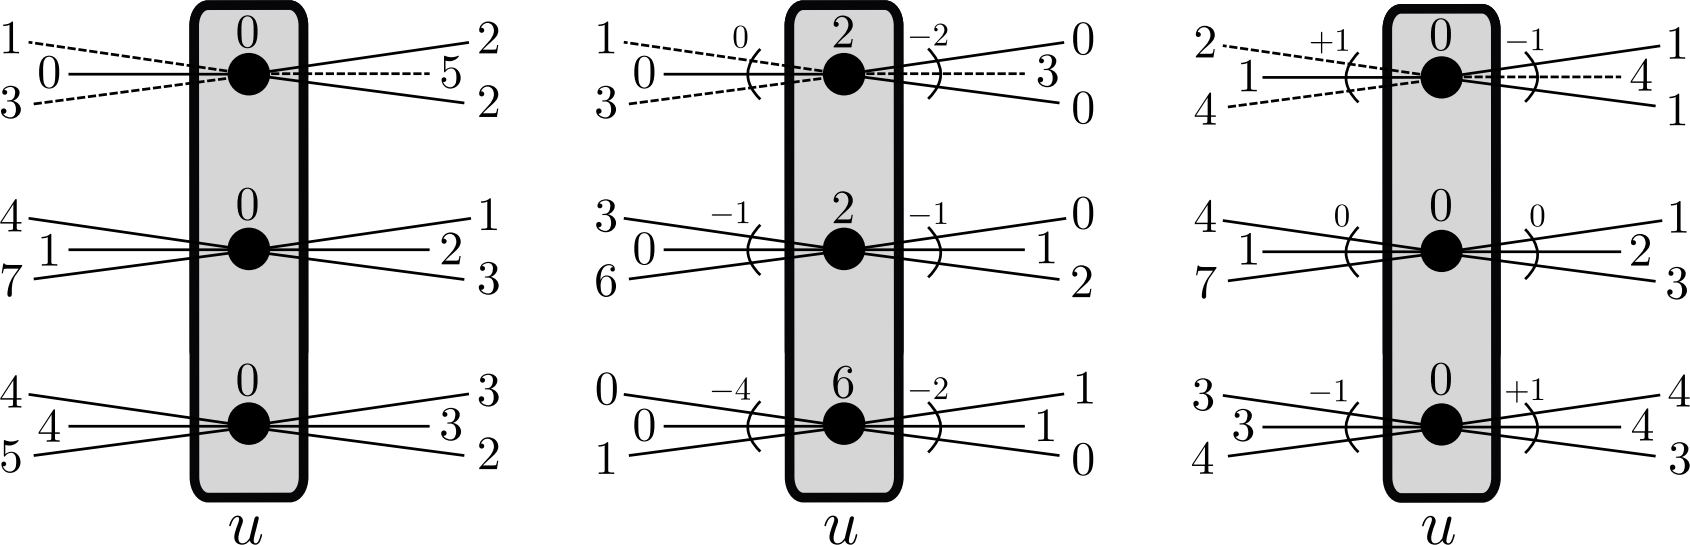
\includegraphics[width=\textwidth]{images/diffusion_step}
  \caption{Приклад виконання елементарного кроку дифузії для вершин в об'єкті $u$.
           На ілюстрації кожна з вершин має по два сусіди.
           Значення репараметризованих штрафів позначені великими числами,
           а значення дуальних змінних $\varphi$~---~меншими.
           Пунктирні лінії позначають мінімальні штрафи за вибір
           дужки від конкретної вершини до кожного сусіднього об'єкта.
           Зліва зображені початкові штрафи,
           посередині~---~штрафи та значення
           двоїстих змінних після виконання кроку \eqref{eq:diffusion:first},
           справа~---~після виконання кроку \eqref{eq:diffusion:second}.
           Зображення взято з монографії \cite{overview:savchynskyy:diffusion}}
  \label{fig:diffusion:step}
\end{figure}

\subsection{Властивості алгоритму дифузії}

Покажемо, що після виконання кожного з перетворень \eqref{eq:diffusion:first}
та \eqref{eq:diffusion:second},
що утворюють елементарний крок алгоритму дифузії,
значення дуальної функції \eqref{eq:lagrange:dual:MAP} не зменшується.

\textbf{Твердження.}
Перший крок алгоритму дифузії \eqref{eq:diffusion:first}
не зменшує значення дуальної функції Лагранжа \eqref{eq:lagrange:dual:MAP}.

Для доведення цього твердження розпишемо цільову функцію задачі
\eqref{eq:lagrange:dual:MAP} після виконання кроку $i + 1$
\begin{equation*}
\begin{gathered}
    \min \limits_{\substack{\pmb{\mu} \in \left\{ 0, 1 \right\}^{\mathcal{I}} \\
                            \pmb{\mu_{\left(x, y \right)}} \in \Delta^{T \times D} \\
                            \pmb{\mu_{\left(x, y \right), \left(x', y' \right)}} \in
                                \Delta^{\mathcal{N} \times D^2}}}
        \langle \pmb{\theta}^{\varphi^{i + 1}}, \pmb{\mu} \rangle = \\
    = \sum \limits_{\left(x, y \right) \in T}
        \min \limits_{d \in D}
            f_{\left(x, y \right)}^{\varphi^{i + 1}} \left( d \right) +
    \sum \limits_{\left( \left(x, y \right), \left(x', y' \right) \right) \in \mathcal{N}}
        \min \limits_{d, d' \in D}
            g_{\left(x, y \right), \left(x', y' \right)}^{\varphi^{i + 1}}
                \left( d, d' \right) =
\end{gathered}
\end{equation*}
Підставимо вирази для репараметризованих штрафів
\eqref{eq:reparametrized:vertex}
та \eqref{eq:reparametrized:edge}
\begin{equation*}
\begin{gathered}
    = \sum \limits_{\left(x, y \right) \in T}
        \min \limits_{d \in D} \left[
            f_{\left(x, y \right)} \left( d \right) -
            \sum \limits_{\left(x', y' \right) \in \mathcal{N} \left(x, y \right)}
                \varphi_{\left(x, y \right), \left(x', y' \right)}^{i + 1}
                    \left( d \right)
        \right] + \\
    + \sum \limits_{\left(\left(x, y \right), \left(x', y' \right) \right) \in \mathcal{N}}
        \min \limits_{d, d' \in D} \left[
            g_{\left(x, y \right), \left(x', y' \right)} \left(d, d' \right) +
            \varphi_{\left(x, y \right), \left(x', y' \right)}^{i + 1}
                \left( d \right) +
            \varphi_{\left(x', y' \right), \left(x, y \right)}^{i + 1}
                \left( d' \right)
        \right] =
\end{gathered}
\end{equation*}
Підставимо вирази для оновлення дуальних змінних на кроці $i + 1$
через дуальні змінні на кроці $i$ \eqref{eq:diffusion:first}
\begin{equation*}
\begin{gathered}
    = \sum \limits_{\left(x, y \right) \in T}
        \min \limits_{d \in D} \left\{
            f_{ \left(x, y \right)} \left(d \right) -
            \sum \limits_{\left(x', y' \right) \in \mathcal{N} \left(x, y \right)}
            \left[
                \varphi_{ \left(x, y \right), \left(x', y' \right)}^i
                    \left(d \right) -
                \min \limits_{d' \in D}
                    g_{\left(x, y \right), \left(x', y' \right)}^{\varphi^i}
                        \left( d, d' \right)
            \right]
        \right\} + \\
    + \sum \limits_{\left(\left(x, y \right), \left(x', y' \right) \right) \in \mathcal{N}}
        \min \limits_{d, d' \in D} \left[ \phantom{\min \limits_{d'' \in D}}
            g_{\left(x, y \right), \left(x', y' \right)} \left(d, d' \right) + \right. \\
            + \varphi_{\left(x, y \right), \left(x', y' \right)}^i
                \left(d \right) -
            \min \limits_{d'' \in D}
                g_{\left(x, y \right), \left(x', y' \right)}^{\varphi^i}
                    \left(d, d'' \right) + \\
            \left. + \varphi_{\left(x', y' \right), \left(x, y \right)}^i
                \left(d' \right) -
            \min \limits_{d'' \in D}
                g_{\left(x', y' \right), \left(x, y \right)}^{\varphi^i}
                    \left(d', d'' \right)
        \right] =
\end{gathered}
\end{equation*}
Внесемо сумму в дужки в першому доданку,
а в другому застосуємо формулу для репараметризованого
штрафу за вибір пари міток на кроці $i$ \eqref{eq:reparametrized:edge}
\begin{equation*}
\begin{gathered}
    = \sum \limits_{\left(x, y \right) \in T}
        \min \limits_{d \in D} \left[
            f_{\left(x, y \right)} \left( d \right) -
            \sum \limits_{\left(x', y' \right) \in \mathcal{N} \left(x, y \right)}
                \varphi_{\left(x, y \right), \left(x', y' \right)}^i
                    \left(d \right) + \right. \\
                \left. + \sum \limits_{\left(x', y' \right) \in \mathcal{N} \left(x, y \right)}
                \min \limits_{d' \in D}
                    g_{\left(x, y \right), \left(x', y' \right)}^{\varphi^i}
                        \left(d, d' \right)
        \right] + \\
    + \sum \limits_{\left(\left(x, y \right), \left(x', y' \right)\right)\in\mathcal{N}}
        \min \limits_{d,d' \in D} \left[
            g_{\left(x, y \right), \left(x', y' \right)}^{\varphi^i}
                \left(d, d' \right) -
            \min \limits_{d'' \in D}
                g_{\left(x, y \right), \left(x', y' \right)}^{\varphi^i}
                    \left(d, d'' \right) - \right. \\
            \left. - \min \limits_{d'' \in D}
                g_{\left(x', y' \right), \left(x, y \right)}^{\varphi^i}
                    \left(d', d'' \right)
        \right] \ge
\end{gathered}
\end{equation*}
В першому доданку
застосуємо формулу для репараметризованого штрафу за вибір вершини з міткою $d$
в об'єкті $\left(x, y \right)$ на кроці $i$ \eqref{eq:reparametrized:vertex},
а в другому доданку скористаємось тим фактом,
що сума мінімумів функцій не перевищує мінімуму суми функцій
\begin{equation*}
\begin{gathered}
    \ge \sum \limits_{\left(x, y \right) \in T}
        \sum \limits_{d \in D} \left[
            f_{\left(x, y \right)}^{\varphi^i} \left(d \right) +
            \sum \limits_{\left(x', y' \right) \in \mathcal{N} \left(x, y \right)}
                \min \limits_{d' \in D}
                    g_{\left(x, y \right), \left(x', y' \right)}^{\varphi^i}
                        \left(d, d' \right)
        \right] + \\
    + \sum \limits_{\left(\left(x, y \right), \left(x', y' \right) \right)\in \mathcal{N}}
    \left[
        \min\limits_{d, d' \in D}
            g_{\left(x, y \right), \left(x', y' \right)}^{\varphi^i}
                \left(d, d' \right) -
        \min\limits_{d, d' \in D}
            g_{\left(x, y \right), \left(x', y' \right)}^{\varphi^i}
                \left(d, d' \right) - \right. \\
        \left. - \min\limits_{d, d' \in D}
            g_{\left(x', y' \right), \left(x, y \right)}^{\varphi^i}
                \left(d', d \right)
    \right] \ge
\end{gathered}
\end{equation*}
Тепер у першому доданку скористаємось тим фактом,
що сума мінімумів функцій не перевищує мінімуму суми функцій.
Також зазначимо, що через те, що дуги в графі не направлені,
має місце рівність
\begin{equation*}
    g_{\left(x, y \right), \left(x', y' \right)}^{\varphi^i}
            \left(d, d' \right) =
    g_{\left(x', y' \right), \left(x, y \right)}^{\varphi^i}
            \left(d', d \right),
\end{equation*}
тому ці штрафи знищуються в другому доданку
\begin{equation*}
\begin{gathered}
    \ge \sum \limits_{\left(x, y \right) \in T} \left[
        \min \limits_{d \in D}
            f_{\left(x, y \right)}^{\varphi^i} \left(d \right) +
        \min \limits_{d \in D}
            \sum \limits_{\left(x', y' \right) \in \mathcal{N} \left(x, y \right)}
                \min \limits_{d' \in D}
                    g_{\left(x, y \right), \left(x', y' \right)}^{\varphi^i}
                        \left(d, d' \right)
    \right] - \\
    - \sum \limits_{\left(\left(x, y \right), \left(x', y' \right) \right) \in \mathcal{N}}
        \min \limits_{d, d' \in D}
            g_{\left(x, y \right), \left(x', y' \right)}^{\varphi^i}
                \left(d, d' \right) \ge
\end{gathered}
\end{equation*}
В першому доданку поміняємо місцями знак суми по сусіднім об'єктам
$\left(x', y' \right) \in \mathcal{N} \left(x, y \right)$
та знак мінімума по міткам $d \in D$ та розкриємо дужки
\begin{equation*}
\begin{gathered}
    \ge \sum \limits_{\left(x, y \right) \in T}
        \min \limits_{d \in D}
            f_{\left(x, y \right)}^{\varphi^i} \left( d \right) +
    \sum \limits_{\left(x, y \right) \in T}
        \sum \limits_{\left(x', y' \right) \in \mathcal{N} \left(x, y \right)}
            \min \limits_{d, d' \in D}
                g_{\left(x, y \right), \left(x', y' \right)}
                    \left( d, d' \right) - \\
    - \sum \limits_{\left(\left(x, y \right), \left(x', y' \right) \right) \in \mathcal{N}}
        \min \limits_{d, d' \in D}
            g_{\left(x, y \right), \left(x', y' \right)} \left( d, d' \right) =
\end{gathered}
\end{equation*}
Другий доданок містить кожну дужку
$\left( \left(x, y \right), \left(x', y' \right) \right)$ два рази,
бо об'єкт $\left(x', y' \right)$ є сусіднім для об'єкта $\left(x, y \right)$,
а об'єкт $\left(x, y \right)$ в свою чергу є сусіднім для об'єкта
$\left(x', y' \right)$
\begin{equation*}
\begin{gathered}
    = \sum \limits_{\left(x, y \right) \in T}
        \min \limits_{d \in D}
            f_{\left(x, y \right)}^{\varphi^i} \left( d \right) +
    \sum \limits_{\left(\left(x, y \right), \left(x', y' \right) \right) \in \mathcal{N}}
        \min \limits_{d, d' \in D}
            g_{\left(x, y \right), \left(x', y' \right)} \left( d, d' \right) = \\
    = \min \limits_{\substack{\pmb{\mu} \in \left\{ 0, 1 \right\}^{\mathcal{I}} \\
                            \pmb{\mu_{\left(x, y \right)}} \in \Delta^{T \times D} \\
                            \pmb{\mu_{\left(x, y \right), \left(x', y' \right)}} \in
                                \Delta^{\mathcal{N} \times D^2}}}
        \langle \pmb{\theta}^{\varphi^i}, \pmb{\mu} \rangle.
\end{gathered}
\end{equation*}
Отримали нерівність
\begin{equation*}
    \min \limits_{\substack{\pmb{\mu} \in \left\{ 0, 1 \right\}^{\mathcal{I}} \\
                            \pmb{\mu_{\left(x, y \right)}} \in \Delta^{T \times D} \\
                            \pmb{\mu_{\left(x, y \right), \left(x', y' \right)}} \in
                                \Delta^{\mathcal{N} \times D^2}}}
        \langle \pmb{\theta}^{\varphi^{i + 1}}, \pmb{\mu} \rangle \ge
    \min \limits_{\substack{\pmb{\mu} \in \left\{ 0, 1 \right\}^{\mathcal{I}} \\
                            \pmb{\mu_{\left(x, y \right)}} \in \Delta^{T \times D} \\
                            \pmb{\mu_{\left(x, y \right), \left(x', y' \right)}} \in
                                \Delta^{\mathcal{N} \times D^2}}}
        \langle \pmb{\theta}^{\varphi^i}, \pmb{\mu} \rangle,
\end{equation*}
тобто крок \eqref{eq:diffusion:first}
алгоритму дифузії не зменшує дуальную функцію Лагранжа \eqref{eq:lagrange:dual:MAP}.

\textbf{Твердження.}
Другий крок алгоритму дифузії \eqref{eq:diffusion:second}
не зменшує значення дуальної функції Лагранжа \eqref{eq:lagrange:dual:MAP}.

Для доведення цього твердження розпишемо цільову функцію задачі
\eqref{eq:lagrange:dual:MAP} після виконання кроку $i + 2$
\begin{equation*}
\begin{gathered}
    \min \limits_{\substack{\pmb{\mu} \in \left\{ 0, 1 \right\}^{\mathcal{I}} \\
                            \pmb{\mu_{\left(x, y \right)}} \in \Delta^{T \times D} \\
                            \pmb{\mu_{\left(x, y \right), \left(x', y' \right)}} \in
                                \Delta^{\mathcal{N} \times D^2}}}
        \langle \pmb{\theta}^{\varphi^{i + 2}}, \pmb{\mu} \rangle = \\
    = \sum \limits_{\left(x, y \right) \in T}
        \min \limits_{d \in D}
            f_{\left(x, y \right)}^{\varphi^{i + 2}} \left( d \right) +
    \sum \limits_{\left( \left(x, y \right), \left(x', y' \right) \right) \in \mathcal{N}}
        \min \limits_{d, d' \in D}
            g_{\left(x, y \right), \left(x', y' \right)}^{\varphi^{i + 2}}
                \left( d, d' \right) =
\end{gathered}
\end{equation*}
Підставимо вирази для репараметризованих штрафів \eqref{eq:reparametrized:vertex}
та \eqref{eq:reparametrized:edge}
\begin{equation*}
\begin{gathered}
    = \sum \limits_{\left(x, y \right) \in T}
        \min \limits_{d \in D} \left[
            f_{\left(x, y \right)} \left(d \right) -
            \sum \limits_{\left(x', y' \right) \in \mathcal{N} \left(x, y \right)}
                \varphi_{\left(x, y \right), \left(x', y' \right)}^{i + 1}
                    \left( d \right)
        \right] + \\
    + \sum \limits_{\left(\left(x, y \right), \left(x', y' \right) \right) \in  \mathcal{N}}
        \min \limits_{d, d' \in D} \left[
            g_{\left(x, y \right), \left(x', y' \right)} \left(d, d' \right) +
            \varphi_{\left(x, y \right), \left(x', y' \right)}^{i + 2}
                \left( d \right) +
            \varphi_{\left(x', y' \right), \left(x, y \right)}^{i + 2}
                \left( d' \right)
        \right] =
\end{gathered}
\end{equation*}
Підставимо вирази для оновлення потенціалів $\varphi$ на кроці $i + 2$
через потенціали на кроці $i + 1$ \eqref{eq:diffusion:second}
\begin{equation*}
\begin{gathered}
    = \sum \limits_{\left(x, y \right) \in T}
        \min \limits_{d \in D} \left\{
            f_{ \left(x, y \right)} \left( d \right) -
            \sum \limits_{\left(x', y' \right) \in \mathcal{N}\left(x, y \right)}
            \left[
                \varphi_{\left(x, y \right), \left(x', y' \right)}^{i + 1}
                    \left( d \right) +
                \frac{f_{\left(x, y \right)}^{\varphi^{i + 1}} \left( d \right)}{\left| \mathcal{N} \left(x, y \right) \right|}
            \right]
        \right\} + \\
    + \sum \limits_{\left( \left(x, y \right), \left(x', y' \right) \right) \in \mathcal{N}}
        \min \limits_{d, d' \in D} \left[
            g_{\left(x, y \right), \left(x', y' \right)} \left( d, d' \right) +
            \varphi_{\left(x, y \right), \left(x', y' \right)}^{i + 1}
                \left( d \right) +
            \frac{f_{\left( x, y \right)}^{\varphi^{i + 1}} \left( d \right)}{\left| \mathcal{N}\left( x, y \right) \right|}
            + \right. \\
            \left. + \varphi_{\left(x', y' \right), \left(x, y \right)}^{i + 1}
                \left( d' \right) +
            \frac{f_{\left( x', y' \right)}^{\varphi^{i + 1}} \left( d' \right)}{\left| \mathcal{N}\left( x', y' \right) \right|}
        \right] =
\end{gathered}
\end{equation*}
В першому доданку розкриємо дужки,
а в другому застосуємо формулу для репараметризованого штрафу за вибір пари
міток на кроці $i + 1$
\eqref{eq:reparametrized:edge}
\begin{equation*}
\begin{gathered}
    = \sum \limits_{\left(x, y \right) \in T}
        \min \limits_{d \in D} \left[
            f_{\left(x, y \right)} \left( d \right) -
            \sum \limits_{\left(x' ,y' \right) \in \mathcal{N}\left( x, y \right)}
                \varphi_{\left(x, y \right), \left(x', y' \right)}^{i + 1}
                    \left( d \right) -
            \sum \limits_{\left(x', y' \right) \in \mathcal{N}\left( x, y \right)}
                \frac{f_{\left( x, y \right)}^{\varphi^{i + 1}}\left( d \right)}{\left|\mathcal{N}\left(x, y \right) \right|}
        \right] + \\
    + \sum \limits_{\left( \left(x, y \right), \left(x', y' \right) \right) \in \mathcal{N}}
        \min \limits_{d, d' \in D} \left[
            g_{\left(x, y \right), \left(x', y' \right)}^{\varphi^{i + 1}}
                \left( d, d'\right) +
            \frac{f_{\left(x, y \right)}^{\varphi^{i + 1}}\left( d \right)}{\left| \mathcal{N}\left(x, y \right) \right|} +
            \frac{f_{\left(x', y' \right)}^{\varphi^{i + 1}}\left( d' \right)}{\left| \mathcal{N}\left(x', y' \right) \right|}
        \right] \ge
\end{gathered}
\end{equation*}
В першому доданку використаємо формулу для репараметризованого штрафу за вибір
мітки на кроці $i + 1$ \eqref{eq:reparametrized:edge},
а в другому доданку внесемо знак мінімума в дужки
\begin{equation*}
\begin{gathered}
    \ge \sum \limits_{\left(x, y \right) \in T}
        \min \limits_{d \in D} \left[
            f_{\left(x, y \right)}^{\varphi^{i + 1}} \left( d \right) -
            \sum \limits_{\left(x', y' \right) \in \mathcal{N}\left(x, y \right)}
                \frac{f_{\left(x, y \right)}^{\varphi^{i + 1}}}{\left| \mathcal{N}\left(x. y \right) \right|}
        \right] + \\
    + \sum \limits_{\left(\left(x, y \right), \left(x', y' \right)\right)\in \mathcal{N}}
    \left[
        \min\limits_{d, d' \in D}
            g_{\left(x, y \right),\left(x', y'\right)}^{\varphi^{i + 1}}
                \left(d, d' \right) +
        \min \limits_{d \in D}
            \frac{f_{\left(x, y \right)}^{\varphi^{i + 1}} \left( d \right)}{\left| \mathcal{N}\left(x, y\right)\right|} +
        \min \limits_{d' \in D}
            \frac{f_{\left(x', y' \right)}^{\varphi^{i + 1}} \left( d' \right)}{\left| \mathcal{N}\left(x', y'\right)\right|}
    \right] \ge
\end{gathered}
\end{equation*}
Розкриємо дужки в обох доданках
\begin{equation*}
\begin{gathered}
    \ge \sum \limits_{\left(x, y \right) \in T}
        \min \limits_{d \in D}
            f_{\left(x, y \right)}^{\varphi^{i + 1}}\left( d \right) -
    \sum \limits_{\left(x, y \right) \in T}
        \min \limits_{d \in D}
            \sum \limits_{\left(x', y' \right) \in \mathcal{N} \left(x, y \right)}
                \frac{f_{\left(x, y \right)}^{\varphi^{i + 1}} \left( d \right)}{\left| \mathcal{N}\left(x, y \right) \right|} + \\
    + \sum \limits_{\left(\left(x, y \right), \left(x', y' \right) \right)\in\mathcal{N}}
        \min \limits_{d, d' \in D}
            g_{\left(x, y \right), \left(x', y' \right)}^{\varphi^{i + 1}}
                \left(d, d' \right) +
    \sum \limits_{\left(\left(x, y \right), \left(x', y' \right) \right)\in\mathcal{N}}
        \min \limits_{d \in D}
            \frac{f_{\left(x, y \right)}^{\varphi^{i + 1}} \left( d \right)}{\left| \mathcal{N}\left(x, y\right)\right|} + \\
    + \sum \limits_{\left(\left(x, y \right), \left(x', y' \right) \right)\in\mathcal{N}}
    \min \limits_{d' \in D}
        \frac{f_{\left(x', y' \right)}^{\varphi^{i + 1}} \left( d' \right)}{\left| \mathcal{N}\left(x', y'\right)\right|} =
\end{gathered}
\end{equation*}
Два останні доданки рівні між собою,
а в сумі вони дорівнюють другому доданку за знаком <<мінус>>, отже,
вони знищуються.
Те, що залишилося,
дорівнює дуальній функції Лагранжа \eqref{eq:lagrange:dual:MAP}
на кроці $i + 1$.
Отримали нерівність
\begin{equation*}
    \min \limits_{\substack{\pmb{\mu} \in \left\{ 0, 1 \right\}^{\mathcal{I}} \\
                            \pmb{\mu_{\left(x, y \right)}} \in \Delta^{T \times D} \\
                            \pmb{\mu_{\left(x, y \right), \left(x', y' \right)}} \in
                                \Delta^{\mathcal{N} \times D^2}}}
        \langle \pmb{\theta}^{\varphi^{i + 2}}, \pmb{\mu} \rangle \ge
    \min \limits_{\substack{\pmb{\mu} \in \left\{ 0, 1 \right\}^{\mathcal{I}} \\
                            \pmb{\mu_{\left(x, y \right)}} \in \Delta^{T \times D} \\
                            \pmb{\mu_{\left(x, y \right), \left(x', y' \right)}} \in
                                \Delta^{\mathcal{N} \times D^2}}}
        \langle \pmb{\theta}^{\varphi^{i + 1}}, \pmb{\mu} \rangle,
\end{equation*}
тобто крок \eqref{eq:diffusion:second}
алгоритму дифузії не зменшує дуальную функцію Лагранжа
\eqref{eq:lagrange:dual:MAP}.

Таким чином,
операції \eqref{eq:diffusion:first} і
\eqref{eq:diffusion:second} максимізують дуальну функцію Лагранжа
\eqref{eq:lagrange:dual:MAP} по потенціалам
$\Phi$, а тому мінімізують штрафну функцію \eqref{eq:overview:penalty}
\cite{overview:savchynskyy:diffusion},
що випливає з прямо-двоїстих умов оптимальності.

Алгоритм полягає в ітеративному повторі елементарного кроку дифузії для всіх об'єктів
$\left(x, y \right) \in T$ до виконання критерію зупинки.
Прикладом критерію зупинки алгоритму може бути мале збільшення
значення дуальної функції Лагранжа \eqref{eq:lagrange:dual:MAP}
\begin{equation*}
    \min \limits_{\substack{\pmb{\mu} \in \left\{ 0, 1 \right\}^{\mathcal{I}} \\
                            \pmb{\mu_{\left(x, y \right)}} \in \Delta^{T \times D} \\
                            \pmb{\mu_{\left(x, y \right), \left(x', y' \right)}} \in
                                \Delta^{\mathcal{N} \times D^2}}}
        \langle \pmb{\theta}^{\varphi^{i + 1}}, \pmb{\mu} \rangle -
    \min \limits_{\substack{\pmb{\mu} \in \left\{ 0, 1 \right\}^{\mathcal{I}} \\
                            \pmb{\mu_{\left(x, y \right)}} \in \Delta^{T \times D} \\
                            \pmb{\mu_{\left(x, y \right), \left(x', y' \right)}} \in
                                \Delta^{\mathcal{N} \times D^2}}}
        \langle \pmb{\theta}^{\varphi^i}, \pmb{\mu} \rangle \le \varepsilon,
\end{equation*}
де $\varepsilon \in \mathbb{R}_+$~---~мале число.
Виконання цього критерію означає,
що ми наблизилися до шуканого максимуму дуальної функції Лагранжа
або потрапили на нерухому точку алгоритму.

\section{Вибір найкращої розмітки}

Після мінімізації енергії задачі \eqref{eq:overview:penalty}
треба знайти одну з тих розміток, штраф яких дорівнює мінімальному штрафу.
Для цього використовується \textit{алгоритм викреслювання другого порядку}
(relaxation labeling algorithm) \cite{overview:savchynskyy:diffusion}.

Розглядається той самий $\left| T \right|$-дольний граф,
в кожній долі (об'єкті) якого міститься $\left| D \right|$ вершин.
Вага вершини з міткою $d \in D$ в об'єкті $\left(x, y \right) \in T$
тепер дорівнює
$\mu_{\left(x, y \right)} \left( d \right) \in \left\{ 0, 1 \right\}$,
а вага дужки між парою міток $d \in D$ в об'єкті $\left( x, y \right) \in T$
та $d' \in D$ в об'єкті $\left(x', y' \right) \in \mathcal{N} \left(x, y \right)$~---~$\mu_{\left(x, y \right), \left(x', y' \right)} \left(d, d' \right)$.

Вершина $\left(x, y, d \right)$ вважається \textit{допустимою},
якщо відповідна їй змінна $\mu_{\left(x, y \right)} \left( d \right) = 1$.
Аналогічно,
пара вершин $\left( \left( x, y, d \right), \left(x', y', d' \right) \right)$
вважається \textit{допустимою}, якщо відповідна змінна
$\mu_{\left(x, y \right), \left(x', y' \right)} \left(d, d' \right) = 1$.

На побудованому графі розв'язується
$\left( \bigvee, \bigwith \right)$-задача, що полягає у відповіді на питання
<<Чи існує така розмітка, при якій всі мітки та пари міток є допустимими?>>.

На початку всі вершини вважаються допустимими, тобто
$\mu_{\left(x, y \right)} \left(d \right) = 1$ для всіх
міток $d \in D$ в кожному об'єкті $\left(y,x \right) \in T$.
В кожній парі сусідніх об'єктів
$\left( \left(x, y \right), \left(x', y' \right) \right) \in \mathcal{N}$
знаходиться дужка з мінімальною вагою
$\min \limits_{d, d' \in D} g_{\left(x, y \right), \left(x', y' \right)}
    \left(d, d' \right) =
    g_{\left(x, y \right), \left(x', y' \right)}
        \left(\tilde{d}, \tilde{d'} \right)$.
Між цією парою об'єктів допустимими є ті дужки,
вага яких відрізняється від мінімальної не більше
наперед заданої малої величини $\varepsilon \in \mathbb{R}_+$
(рис. \ref{fig:epsilon:edges}), тобто
$\mu_{\left(x, y \right), \left(x', y' \right)} \left(d, d' \right) = 1$,
якщо
\begin{equation*}
    g_{\left(x, y \right), \left(x', y' \right)} \left(d, d' \right) -
    g_{\left(x, y \right), \left(x', y' \right)}
        \left(\tilde{d}, \tilde{d'} \right) \le
    \varepsilon.
\end{equation*}
Якщо ця нерівність не виконується, дужка вважається не допустимою,
відповідна змінна
$\mu_{\left(x, y \right), \left(x', y' \right)} \left(d, d' \right) = 0$.

\begin{figure}[h]
\centering
    \begin{subfigure}[t]{0.475\textwidth}
        \centering
        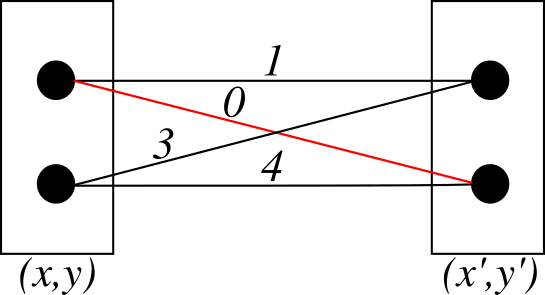
\includegraphics[width=\textwidth]{images/epsilon_edges_min}
        \caption{Штрафи за вибір пари міток між двома сусідніми об'єктами.
                 Дужка з мінімальним штрафом позначена червоним}
        \label{fig:epsilon:edges:min}
    \end{subfigure}
    \hfill
    \begin{subfigure}[t]{0.475\textwidth}
        \centering
        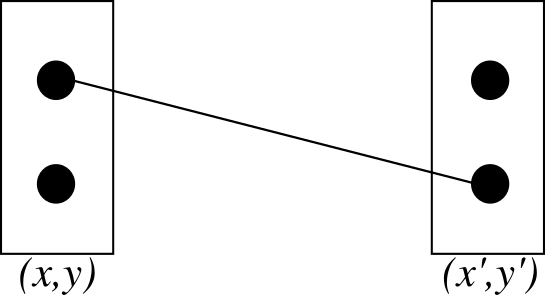
\includegraphics[width=\textwidth]{images/epsilon_edges_05}
        \caption{Допустимі дужки при $\varepsilon = 0.5$}
        \label{fig:epsilon:edges:0.5}
    \end{subfigure}
    \vskip\baselineskip
    \begin{subfigure}[t]{0.475\textwidth}
        \centering
        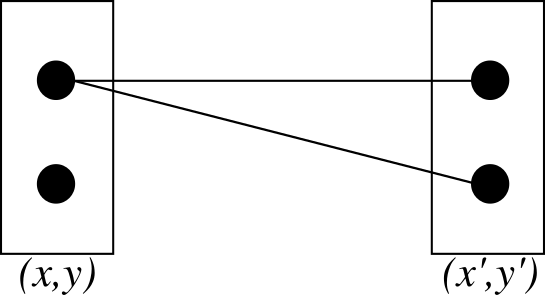
\includegraphics[width=\textwidth]{images/epsilon_edges_1}
        \caption{Допустимі дужки при $\varepsilon = 1$}
        \label{fig:epsilon:edges:1}
    \end{subfigure}
    \quad
    \begin{subfigure}[t]{0.475\textwidth}
        \centering
        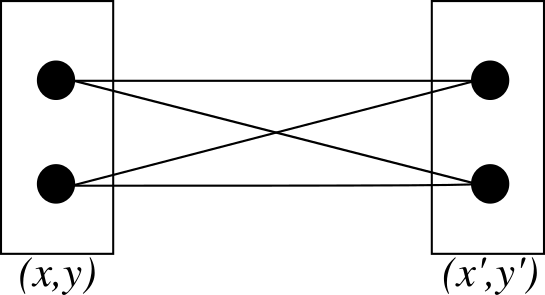
\includegraphics[width=\textwidth]{images/epsilon_edges_4}
        \caption{Допустимі дужки при $\varepsilon = 4$}
        \label{fig:epsilon:edges:4}
    \end{subfigure}
    \caption{Допустимі дужки при різних значеннях $\varepsilon$}
    \label{fig:epsilon:edges}
\end{figure}

Алгоритм полягає в багатократному застосуванні
\textit{операції <<викреслювання вершини>>} (рис. \ref{fig:crossing:vertex})
\begin{equation*}
    \mu_{\left(x, y \right)} \left(d \right)
    = \mu_{\left(x, y \right)} \left(d \right)
    \with \bigwith \limits_{\left(x', y' \right)\in \mathcal{N}\left(x, y \right)}
        \bigvee \limits_{d' \in D}
            \mu_{\left(x, y \right), \left(x', y' \right)}
                \left(d, d' \right)
\end{equation*}
та \textit{операції <<викреслювання дужки>>} (рис. \ref{fig:crossing:edge})
\begin{equation*}
    \mu_{\left(x, y \right), \left(x', y' \right)} \left(d, d' \right)
    = \mu_{\left(x, y \right), \left(x', y' \right)} \left(d, d' \right)
    \with \mu_{\left(x, y \right)} \left(d \right)
    \with \mu_{\left(x', y' \right)} \left(d' \right).
\end{equation*}

\begin{figure}[h]
\centering
    \begin{subfigure}[t]{0.45\textwidth}
        \centering
        \includegraphics[width=\textwidth]{images/crossing_vertex}
        \caption{З вершини $\left(x, y, d \right)$ до об'єкту
                 $\left(x, y \right)$ всі дужки викреслені (не допустимі),
                 тому вершина $\left(x, y, d \right)$ теж стає недопустимою}
        \label{fig:crossing:vertex:yes}
    \end{subfigure}
    \hfill
    \begin{subfigure}[t]{0.45\textwidth}
        \centering
        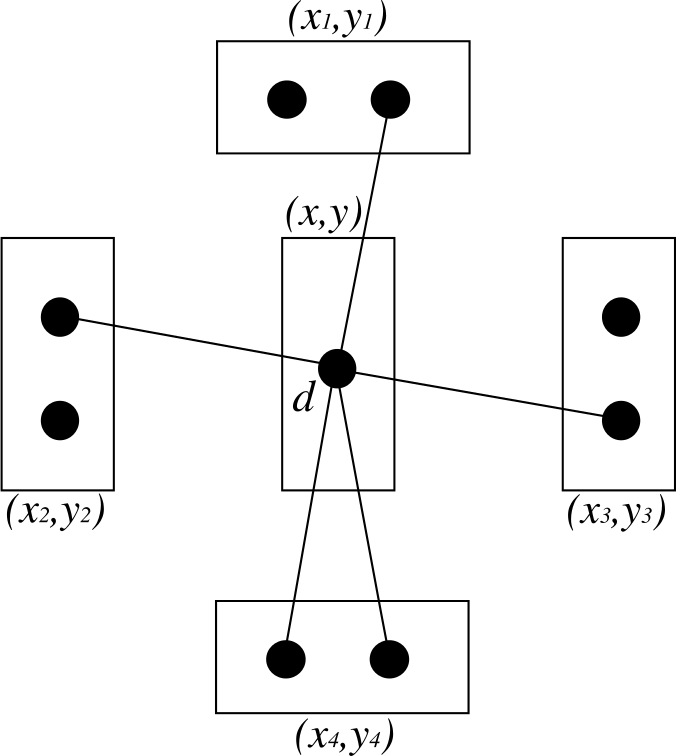
\includegraphics[width=\textwidth]{images/crossing_vertex_no}
        \caption{Вершину $\left(x, y, d \right)$
                 поєднує допустима дужка хоча б з однією
                 вершиною в кожному сусідньому об'єкті.
                 Вершина $\left(x, y, d \right)$ залишається допустимою}
        \label{fig:crossing:vertex:np}
    \end{subfigure}
    \caption{Операція <<викреслювання вершини>>.
             Зображені лише допустимі дужки}
    \label{fig:crossing:vertex}
\end{figure}

\begin{figure}[h]
  \centering
  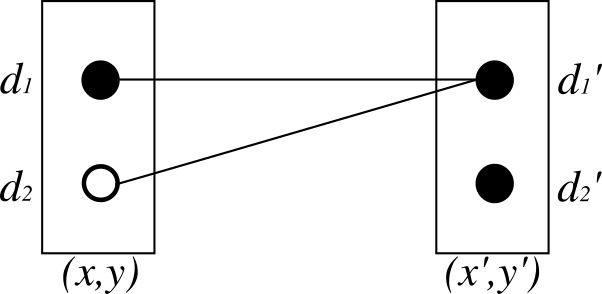
\includegraphics[width=0.6\textwidth]{images/crossing_edge}
  \caption{Операція <<викреслювання дужки>>.
           Зафарбованими кружечками позначені допустимі вершини,
           незафарбованими~---~недопустимі вершини.
           Дужка, що поєднує мітку $d_2$ в об'єкті $\left(x, y\right)$
           та мітку $d_1'$ в об'єкті $\left(x', y' \right)$, буде викреслена,
           бо одна з цих міток, а саме $d_2$, є недопустимою.
           Дужка, що поєднує мітку $d_1$ в об'єкті $\left(x, y\right)$
           та мітку $d_1'$ в об'єкті $\left(x', y' \right)$,
           залишиться допустимою}
  \label{fig:crossing:edge}
\end{figure}

Алгоритм завершує роботу зі скінченну кількість ітерацій,
адже ніяка викреслена вершина або дужка не може знов стати допустимою.
Якщо після завершення роботи алгоритму деякі вершини залишились допустимими,
то було зроблено досить ітерацій дифузії,
і з множини допустимих вершин можна побудувати розмітку.

Таким чином, для знаходження найкращої розмітки, необхідно
\begin{enumerate}
    \item виконати $N$ ітерацій алгоритму дифузії, де $N$~---~фіксоване число;
    \item запустити алгоритм викреслювання другого порядку;
    \item якщо після зупинки алгоритму викреслювання залишились
          допустимі вершини, вибрати найкращу розмітку,
          інакше~---~перейти до першого кроку.
\end{enumerate}

Для гарантії існування
розмітки після застосування алгоритму дифузії штрафи за вибір пари міток $g$
вихідного графу повинні мати властивість субмодулярності
\cite{diffusion:shlezinger:supermodularity}.

Для введення субмодулярності необхідно задати порядок на множині міток $D$.
В задачі стереобачення, яка розглядається, мітки задаються цілими числами,
які можна впорядкувати по зростанню або спаданню.
Будемо вважати, що серед двох міток $d, d' \in D$ \textit{вищою} є та мітка,
значення якої менше, як зображено на рисунку \ref{fig:phi:block}.
Тобто якщо $d < d'$, то $d$ є вищою за $d'$.

\textbf{Означення.}
Функція $g$ є \textit{субмодулярною}, якщо для будь-якої пари сусідніх об'єктів
$\left(\left(x, y \right), \left(x', y' \right) \right) \in \mathcal{N}$
та будь-яких пар міток $d_1 > d_2$ та $d_1' > d_2'$
(рис. \ref{fig:submodular:function}) виконується нерівність
\begin{equation} \label{eq:submodular:function}
\begin{gathered}
    g_{\left(x, y \right), \left(x', y' \right)} \left(d_1, d_1' \right) +
    g_{\left(x, y \right), \left(x', y' \right)} \left(d_2, d_2' \right) \le \\
    \le g_{\left(x, y \right), \left(x', y' \right)} \left(d_1, d_2' \right) +
    g_{\left(x, y \right), \left(x', y' \right)} \left(d_2, d_1' \right).
\end{gathered}
\end{equation}

\begin{figure}[h]
  \centering
  \includegraphics[width=0.6\textwidth]{images/submodular_function}
  \caption{Для субмодулярної функції сума паралельних дужок (позначені червоним)
           не перевищує суми дужок, що перетинаються (позначені чорним)}
  \label{fig:submodular:function}
\end{figure}

Прикладом штрафної функції для дужок з властивістю субмодулярності
є модуль різниці між значеннями міток
\begin{equation} \label{eq:edge:abs}
    g_{\left(x, y \right), \left(x', y' \right)} \left( d, d' \right)
    = \left| d - d' \right|.
\end{equation}
Для доведення цього твердження достатньо розглянути два сусідніх об'єкта
$\left(\left(x, y \right), \left(x', y' \right) \right) \in \mathcal{N}$
з двома мітками в кожному: $d_1 > d_2$ та $d_1' > d_2'$
та розглянути всі можливі варіанти значень міток
(рис. \ref{fig:submodularity:abs:proof}).
Для всіх можливих випадків, що зображені на рисунку,
необхідно розкрити модулі в нерівності \eqref{eq:submodular:function}
та переконатися, що вони виконуються.

\begin{figure}[h]
  \centering
  \includegraphics[width=0.9\textwidth]{images/submodularity_abs_proof}
  \caption{Ілюстрація для доведення того факту,
           що \eqref{eq:edge:abs}~---~субмодулярна функція}
  \label{fig:submodularity:abs:proof}
\end{figure}

Якщо після того, як алгоритм викреслювання зупинився,
в кожному об'єкті $\left(x, y \right) \in T$
залишилась хоча б одна допустима вершина,
то в кожному об'єкті обирається та мітка, яка є найвищою.
Сукупність таких міток і буде утворювати оптимальну розмітку.

\section*{Висновки до розділу 2}
\addcontentsline{toc}{section}{Висновки до розділу 2}

Пред'явлено розв'язок задачі стереобачення за допомогою алгоритма дифузії.
Доведено, що кожний крок алгоритму дифузії не зменшує дуальну функцію Лагранжа
для енергії задачі, а також наведені інші важливі властивості.
Описано, як знайти оптимальну розмітку після розв'язання задачі оптимізації.
